\documentclass[10pt]{article}
\usepackage[letterpaper,text={6.5in,8.7in},centering]{geometry}
\usepackage{amssymb,amsmath,times,url,subfigure,graphicx,theorem,alltt,eepic,tikz}
%\usepackage[pdftex,urlcolor=blue,pdfpagemode=none,pdfstartview=FitH]{hyperref}

%% url smaller font.
\makeatletter
\def\url@leostyle{%
  \@ifundefined{selectfont}{\def\UrlFont{\sf}}{\def\UrlFont{\small\ttfamily}}}
\makeatother
\urlstyle{leo}

%\usepackage[all,import]{xy}

\newcommand{\norm}[1]{\ensuremath{\left\| #1 \right\|}}
\newcommand{\abs}[1]{\ensuremath{\left| #1 \right|}}
\newcommand{\bracket}[1]{\ensuremath{\left[ #1 \right]}}
\newcommand{\braces}[1]{\ensuremath{\left\{ #1 \right\}}}
\newcommand{\parenth}[1]{\ensuremath{\left( #1 \right)}}
\newcommand{\ip}[1]{\ensuremath{\langle #1 \rangle}}
\newcommand{\refeqn}[1]{(\ref{eqn:#1})}
\newcommand{\reffig}[1]{Fig. \ref{fig:#1}}
\newcommand{\tr}[1]{\mbox{tr}\ensuremath{\negthickspace\bracket{#1}}}
\newcommand{\deriv}[2]{\ensuremath{\frac{\partial #1}{\partial #2}}}
\newcommand{\SO}{\ensuremath{\mathrm{SO(3)}}}
\newcommand{\T}{\ensuremath{\mathrm{T}}}
\newcommand{\so}{\ensuremath{\mathfrak{so}(3)}}
\newcommand{\SE}{\ensuremath{\mathrm{SE(3)}}}
\newcommand{\se}{\ensuremath{\mathfrak{se}(3)}}
\renewcommand{\Re}{\ensuremath{\mathbb{R}}}
\renewcommand{\S}{\ensuremath{\mathbb{S}}}
\newcommand{\aSE}[2]{\ensuremath{\begin{bmatrix}#1&#2\\0&1\end{bmatrix}}}
\newcommand{\ase}[2]{\ensuremath{\begin{bmatrix}#1&#2\\0&0\end{bmatrix}}}
\newcommand{\D}{\ensuremath{\mathbf{D}}}
\newcommand{\pair}[1]{\ensuremath{\left\langle #1 \right\rangle}}
\newcommand{\met}[1]{\ensuremath{\langle\!\langle #1 \rangle\!\rangle}}
\newcommand{\Ad}{\ensuremath{\mathrm{Ad}}}
\newcommand{\ad}{\ensuremath{\mathrm{ad}}}
\newcommand{\g}{\ensuremath{\mathfrak{g}}}

\renewcommand{\baselinestretch}{1.2}
\date{}

\renewcommand{\thesubsection}{\arabic{subsection}. }
\renewcommand{\thesubsubsection}{\arabic{subsection}.\arabic{subsubsection} }

\theoremstyle{plain}\theorembodyfont{\normalfont}
\newtheorem{prob}{Problem}[section]
%\renewcommand{\theprob}{\arabic{section}.\arabic{prob}}
\renewcommand{\theprob}{\arabic{prob}}

\newenvironment{subprob}%
{\renewcommand{\theenumi}{\alph{enumi}}\renewcommand{\labelenumi}{(\theenumi)}\begin{enumerate}}%
{\end{enumerate}}%

\newenvironment{matlab}
{\begin{alltt}\small\renewcommand{\baselinestretch}{1.2}\selectfont}%
{\end{alltt}}

\newcommand*\circled[1]{%
  \tikz[baseline=(C.base)]\node[draw,circle,inner sep=0.5pt](C) {#1};\!
}

\begin{document}

\pagestyle{empty}
\section*{MAE3145: Homework 4}
\vspace*{-0.4cm}
\noindent{Due date: November 9, 2016}%\\%\vspace*{0.5cm}

%\begin{prob}
%We will compare the cost of a Hohmann transfer between circular orbits with the cost of a bi-elliptic Hohmann transfer between the same orbits. Assume that $\mu=398600\,\mathrm{km^3/s^2}$.
%
%\begin{subprob}
%
%\item Consider a Hohmann transfer from a circular orbit with radius $r_A=8000\,\mathrm{km}$ to another circular orbit with radius $r_C=104000\,\mathrm{km}$. Find the required total velocity change, and the transfer time.
%
%\item Consider a bi-elliptic Hohmann transfer between the above orbits in (a) with an intermediate apoapsis radius of $r_B=160000\,\mathrm{km}$. Find the required total velocity change, and the transfer time. Compare these with your solution of (a).
%
%\item The following Matlab function, \texttt{Hohmann.m} computes the total velocity change and the transfer time of a Hohmann transfer for given $r_A,r_C$. 
%\begin{matlab}
%function [delV delT]=Hohmann(rA,rC)
%mu=398600;
%
%VA1=sqrt(mu/rA);
%VA2=sqrt(2*mu/(rA+rC)*rC/rA);
%delVA=VA2-VA1;
%
%VC2=sqrt(2*mu/(rA+rC)*rA/rC);
%VC3=sqrt(mu/rC);
%delVC=VC3-VC2;
%
%delV=abs(delVA)+abs(delVC);
%
%a2=1/2*(rA+rC);
%T2=2*pi/sqrt(mu)*a2^(3/2);
%delT=T2/2;
%\end{matlab}
%
%Compose a Matlab function, \texttt{BEHohmann.m} that computes the total cost and transfer time of a bi-elliptic Hohmann transfer for given $r_A,r_B,r_C$. The first few lines of this Matlab function are as follows.
%\begin{matlab}
%1: function [delV delT]=BEHohmann(rA,rB,rC);
%2: mu=398600;
%3: 
%4: VA1=sqrt(mu/rA);
%5: VA2=sqrt(2*mu/(rA+rB)*rB/rA);
%6: delVA=VA2-VA1;
%\end{matlab}
%Check that this Matlab function gives your solution of (b).
%
%
%\newpage
%
%\item We wish to find a condition on $r_B$ that makes the bi-elliptic Hohmann transfer more efficient. Let $\Delta V_H$, and $\Delta V_B$ be the total velocity change of the Hohmann transfer and the bi-elliptic Hohmann transfer, respectively. Plot $\frac{\Delta V_B}{\Delta V_H}$ with respect to $\frac{r_B}{r_A}$ when $r_B$ is varying from $10r_A$ and $60r_A$, i.e. \texttt{rB=linspace(rA*10,rA*60,500);}. The resulting plot will be similar to the following figure:\\
%
%\centerline{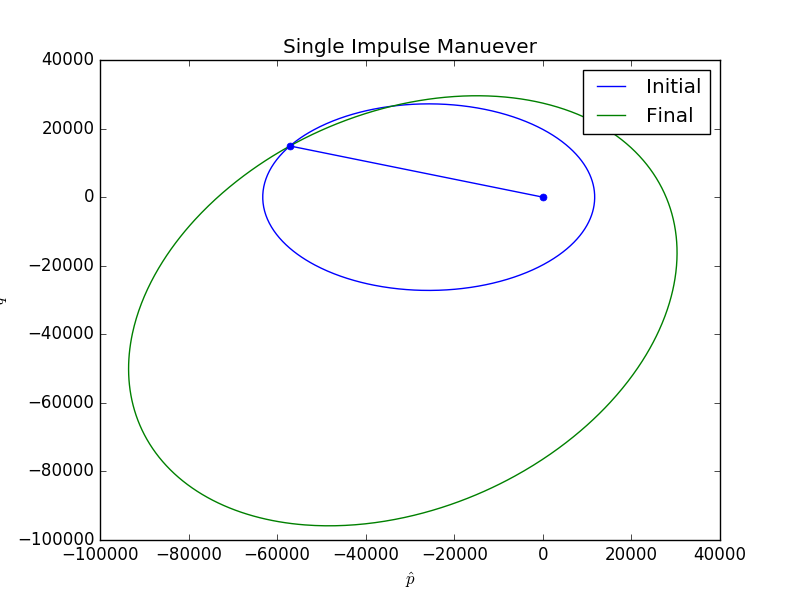
\includegraphics[width=0.45\textwidth]{prob1.eps}}
%
%\item At the above figure, if $\frac{r_B}{r_A}$ is greater than a certain value, which is denoted by a red star, then $\frac{\Delta V_B}{\Delta V_H}< 1$, i.e., the bi-elliptic Hohmann transfer is more efficient than the Hohmann transfer. From your figure, determine the value of $\frac{r_B}{r_A}$ at the red star. In other words, we have
%\begin{align*}
%\frac{r_B}{r_A}\geq c \quad\Rightarrow \quad \frac{\Delta V_B}{\Delta V_H}< 1,
%\end{align*}
%for a constant $c$. What is the minimum possible value of $c$? (try to read your graph as best you can.)
%
%%From your figure, determine when the bi-elliptic Hohmann transfer is more efficient, i.e. find a condition on $\frac{r_B}{r_A}$ such that $\frac{\Delta V_B}{\Delta V_H}< 1$.
%\end{subprob}
%
%\end{prob}



\begin{prob}
A satellite is on a circular orbit with the orbital radius of $r_P=7000\,\mathrm{km}$. We wish to design an impulsive maneuver such that the orbital radius is increased to $r_A=9000\,\mathrm{km}$. Assume $\mu=398600\,\mathrm{km^3/s^2}$. 
\begin{subprob}
\item Show that the initial impulse for the Hohman transfer is $\Delta v_P = 0.4577\,\mathrm{km/s}$.
\item Show that the terminal impulse for the Hohman transfer is $\Delta v_A = 0.4298\,\mathrm{km/s}$.
\item Find the total velocity change $\Delta v_{total}$ and the transfer time $t_{PA}$. 
\end{subprob}
\end{prob}

\begin{prob}
We wish to simulate the above Hohmann transfer using STK. You may follow the steps described below, and upload the resulting \texttt{jpg} file to Blackboard. 

\paragraph{First Impulse}

\begin{list}{$\bullet$}
{\setlength{\itemsep}{-3pt}\setlength{\leftmargin}{30pt}}
\item Download \emph{Hohmann.zip} from Black Board, and extract it to a folder.

(\textcolor{red}{Note: You SHOULD EXTRACT all of the files to your folder!} Double-clicking the scenario file from the zip folder prevents loading predefined satellite.)

\item Open \emph{Hohmann.sc}
\item Double-click \emph{GWU\_Sat}, then the \emph{Basic Orbit} window appears
\item Click the icon for \emph{Insert Segment}, then the \emph{Segment Section} window appears
\item Select \emph{Maneuver} and click \emph{Ok}
\item Type \textcolor{red}{\emph{0.4577}} at \emph{Delta V Magnitude} and click \emph{Apply}
\item Click the icon for \emph{Insert Segment}, then the \emph{Segment Section} window appears
\item Select \emph{Propagate} and click \emph{Ok}
\item Uncheck \emph{Duration}
\item Click \emph{Insert} and choose \emph{Apoapsis}
\item Click the icon for \emph{Run Entire Mission Control Sequence}
\item Watch the \emph{2D Graphics Window} and the \emph{3D Graphics Window}
\end{list}

\paragraph{Second Impulse}

\begin{list}{$\bullet$}
{\setlength{\itemsep}{-3pt}\setlength{\leftmargin}{30pt}}
\item Double-click \emph{GWU\_Sat}, then the \emph{Basic Orbit} window appears
\item Click the icon for \emph{Insert Segment}, then the \emph{Segment Section} window appears
\item Select \emph{Maneuver} and click \emph{Ok}
\item Type \textcolor{red}{\emph{0.4298}} at \emph{Delta V Magnitude} and click \emph{Apply}
\item Click the icon for \emph{Insert Segment}, then the \emph{Segment Section} window appears
\item Select \emph{Propagate} and click \emph{Ok}
\item Click the icon for \emph{Run Entire Mission Control Sequence}
\item Watch the \emph{2D Graphics Window} and the \emph{3D Graphics Window}
\item Click the icon for \emph{Snap Frame} at the \emph{3D Graphics Window}, and type the file name and save it as jpg
\item \textcolor{red}{Upload your jpg file to Black Board }
\end{list}


\end{prob}




\begin{prob}
A spacecraft is returning from an interplanetary mission along a hyperbolic orbit, and a space station on a circular orbit, namely Orbit $\footnotesize\circled{4}$\,, around the Earth counter-clockwise. Currently, the spacecraft is at the periapsis of the hyperbolic orbit, the point $A$, and the space station is at the point $B$. At the current time, we set the absolute time $t=0$.

\centerline{
\setlength{\unitlength}{2.5em}\centering\small
\begin{picture}(12,7)(1.5,-3.0)
\put(7,0){\circle{6}}
\put(7.9,0){\ellipse{4.2}{3.79}}
\put(7.7,0){\ellipse{4.6}{4.38}}
\put(3,0){\vector(1,0){8}}
\put(7,0){\vector(0,1){3.5}}
\put(5.8,0){\circle*{0.12}}
\put(10,0){\circle*{0.12}}
\put(5.4,0){\circle*{0.12}}
\put(5.8,1.2){\vector(0,-1){1}}
\put(7,0){\circle*{1.3}}
\linethickness{0.5pt}
\put(5.8,1.4){$v_{A_1}$}
\put(5.6,-0.4){$A$}
\put(10.1,-0.4){$B$}
\put(5.0,-0.4){$C$}
\put(10.80,-0.4){$\vec x$}
\put(7.1,3.2){$\vec y$}
\put(7.9,-1.75){$\scriptsize\circled{2}$}
\put(7.4,-2.5){$\scriptsize\circled{3}$}
\put(6.8,-2.9){$\scriptsize\circled{4}$}
\end{picture}}
\vspace*{-0.8cm}
\begin{gather*}
r_A=7000\,\mathrm{km},\quad r_B=14000\,\mathrm{km},\quad v_{A_1}=12\,\mathrm{km/s},\quad \mu =398600\,\mathrm{km^3/s^2}.
\end{gather*}
We wish to design an orbital maneuver of the spacecraft such that a rendezvous between the spacecraft and the space station occurs at the point B. The maneuver of the spacecraft is composed of the following orbits:

\begin{center}\vspace*{-0.3cm}
{\small\selectfont
\begin{tabular}{|c|c|c|c|c|c|c|}\hline
& Description  & Periapsis & Apoapsis & Velocity at the beginning & Velocity at the end\\\hline
Orbit \circled{1} & Hyperbolic return orbit & $A$ & - & - & $v_{A_1}$ ($t=0$)\\
Orbit \circled{2} & Hohmann transfer from $A$ to $B$ & $A$ & $B$ & $v_{A_2}$  ($t=0$)& $v_{B_2}$  ($t=t_{1}$)\\
Orbit \circled{3} & Phasing orbit from $B$ to $B$ & $C$ & $B$ & $v_{B_3}$ ($t=t_{1}$) & $v_{B_3}$ ($t=t_{2}$)\\
Orbit \circled{4} & Target circular orbit (counter-clockwise) &$B$ & $B$ & $v_{B_4}$ ($t=t_{2}$)& - \\ \hline
\end{tabular}}
\end{center}


\begin{subprob}
\item Find the velocity change at point $A$, namely $\Delta V_{A}=v_{A_2}-v_{A_1}$, to transfer the spacecraft from Orbit \circled{1} to Orbit \circled{2} at $t=0$.
\item Compute the absolute time $t_1$ when the spacecraft arrives at $B$ from Orbit \circled{2}. 
\item Find the location of the space station when $t=t_{1}$ (answer in terms of the angle measured from the $\vec x$ axis counter-clockwise). What is the \textit{absolute} time $t_2$ when the space station returns to $B$.
\item The period of the phasing orbit \circled{3} should be $T_3=t_{2}-t_{1}$. Find the semi-major axis $a_3$, and distance to the apoapsis $r_C$ of the phasing orbit \circled{3}.
\item Find the velocity change at point $B$, namely $\Delta V_{B_1}=v_{B_3}-v_{B_2}$, to transfer the spacecraft from Orbit \circled{2} to Orbit \circled{3} at $t=t_{1}$.
\item Find the velocity change at point $B$, namely $\Delta V_{B_2}=v_{B_4}-v_{B_3}$, to transfer the spacecraft from Orbit \circled{3} to Orbit \circled{4} at $t=t_{2}$.
\item Show that the total velocity change is $\Delta V_{total} = |\Delta V_A| + |\Delta V_{B_1}| +|\Delta V_{B_2}|=4.2657\,\mathrm{km/s}$.
\end{subprob}


\end{prob}

\end{document}

